\subsection{Perancangan Skema \textit{Database}}

	Pada awalnya, database didesain dengan PDM sebagai berikut berikut : 
	
	\begin{figure}[H]
		\centering
		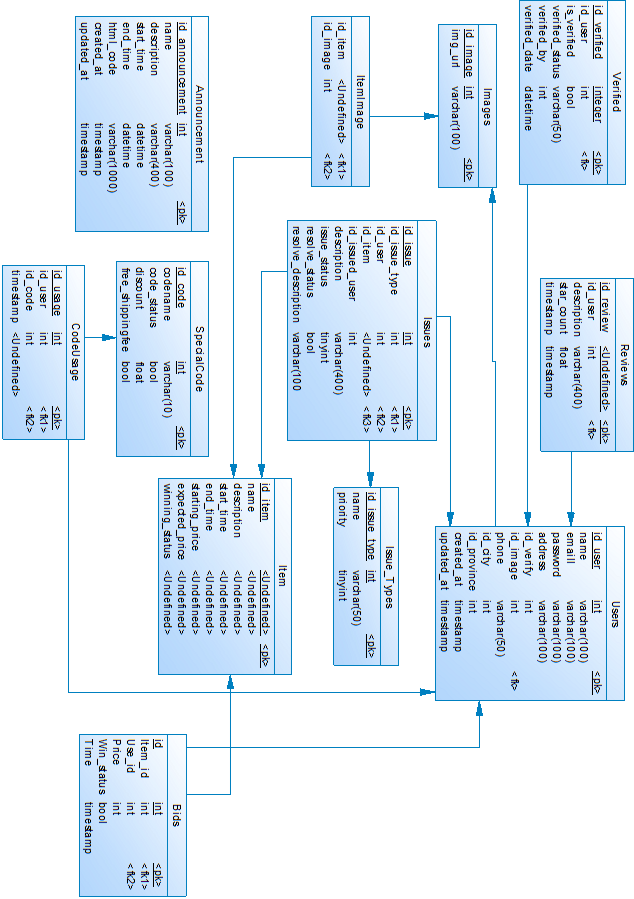
\includegraphics[height=0.6\paperheight]{images/bab3/db/pdm-awal.png}
		\caption{Rancangan Awal PDM untuk Database Relasional}
		\label{pdm-awal}
	\end{figure}
	
	Dan untuk tabel NoSQL dirancang sebagai berikut :
	\begin{figure}[H]
		\centering
		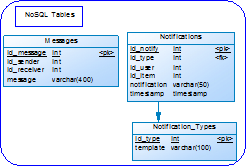
\includegraphics[width=\textwidth]{images/bab3/db/pdm-nosql-awal.png}
		\caption{Rancangan Awal PDM untuk Database Non-Relasional}
		\label{pdm-nosql-awal}
	\end{figure}
	
	Untuk database versi paling \textit{update}, dapat dilihat pada gambar berikut :
	\begin{figure}[H]
		\centering
		
\includegraphics[width=\textwidth]{images/no-image.png}
		\caption{PDM ter\textit{update} untuk Database Relasional}
		\label{pdm-final}
	\end{figure}
	
	Dan untuk tabel NoSQL dirancang sebagai berikut :
	\begin{figure}[H]
		\centering
		
\includegraphics[width=\textwidth]{images/no-image.png}
		\caption{PDM Ter\textit{Update} Database Non-Relasional}
		\label{pdm-nosql-final}
	\end{figure}
	
	Namun, karena pengembangan aplikasi yang bersifat \textit{agile} dan terus berubah karena perkembangan dan \textit{improvization} dari hasil analisa penulis, sifatnya menjadi sangat dinamis.\\

	Berikut akan dipaparkan spesifikasi dan penjelasan setiap tabel.
	\subsubsection{Spesifikasi Tabel User}
	
	\begin{table}[H]
		\centering
		\begin{tabular}{|r|l|l|l|}
			\hline
			\multicolumn{4}{|c|}{\textbf{Tabel items}} \\ \hline
			\textbf{Deskripsi} & \multicolumn{3}{l|}{Tabel ini menyimpan data XX YY ZZ} \\ \hline
			\textbf{Penyimpanan} & \multicolumn{3}{l|}{Transaksional / PostgreSQL} \\ \hline
			\textbf{\begin{tabular}[c]{@{}r@{}}Growth \\ Speed\end{tabular}} & \multicolumn{3}{l|}{\begin{tabular}[c]{@{}l@{}}(masih dipertimbangkan, tapi ini isinya \\ perhitungan/kalkulasi kasar perhitungan \\ penambahan data)\end{tabular}} \\ \hline
			\multicolumn{4}{|c|}{\textbf{Penjelasan Kolom Tabel User}} \\ \hline
			\multicolumn{1}{|l|}{No} & Nama Atribut & Tipe Data & Keterangan \\ \hline
			\begin{tabular}[c]{@{}r@{}}1\\ {[}PK{]}\end{tabular} & ID & INT & \begin{tabular}[c]{@{}l@{}}Autoincrement\\ oleh Sistem\end{tabular} \\ \hline
			2 & Name & varchar(255) & \begin{tabular}[c]{@{}l@{}}Diisi oleh\\ Pengguna\end{tabular} \\ \hline
			\begin{tabular}[c]{@{}r@{}}3\\ {[}FK{]}\end{tabular} & Category\_id & int & Diisi pengguna \\ \hline
			4 & Updated\_at & timestamp & \begin{tabular}[c]{@{}l@{}}Diisi oeh\\ Sistem\end{tabular} \\ \hline
		\end{tabular}
		\caption{Spesifikasi Tabel Z}
		\label{items-tab}
	\end{table}
	
	
		\subsubsection{Spesifikasi Tabel User}
		
		\begin{table}[H]
			\centering
			\begin{tabular}{|r|l|l|l|}
				\hline
				\multicolumn{4}{|c|}{\textbf{Tabel items}} \\ \hline
				\textbf{Deskripsi} & \multicolumn{3}{l|}{Tabel ini menyimpan data XX YY ZZ} \\ \hline
				\textbf{Penyimpanan} & \multicolumn{3}{l|}{Transaksional / PostgreSQL} \\ \hline
				\textbf{\begin{tabular}[c]{@{}r@{}}Growth \\ Speed\end{tabular}} & \multicolumn{3}{l|}{\begin{tabular}[c]{@{}l@{}}(masih dipertimbangkan, tapi ini isinya \\ perhitungan/kalkulasi kasar perhitungan \\ penambahan data)\end{tabular}} \\ \hline
				\multicolumn{4}{|c|}{\textbf{Penjelasan Kolom Tabel User}} \\ \hline
				\multicolumn{1}{|l|}{No} & Nama Atribut & Tipe Data & Keterangan \\ \hline
				\begin{tabular}[c]{@{}r@{}}1\\ {[}PK{]}\end{tabular} & ID & INT & \begin{tabular}[c]{@{}l@{}}Autoincrement\\ oleh Sistem\end{tabular} \\ \hline
				2 & Name & varchar(255) & \begin{tabular}[c]{@{}l@{}}Diisi oleh\\ Pengguna\end{tabular} \\ \hline
				\begin{tabular}[c]{@{}r@{}}3\\ {[}FK{]}\end{tabular} & Category\_id & int & Diisi pengguna \\ \hline
				4 & Updated\_at & timestamp & \begin{tabular}[c]{@	{}l@{}}Diisi oeh\\ Sistem\end{tabular} \\ \hline
			\end{tabular}
			\caption{Spesifikasi Tabel Z}
			\label{items-2tab}
		\end{table}
	